% Options for packages loaded elsewhere
\PassOptionsToPackage{unicode}{hyperref}
\PassOptionsToPackage{hyphens}{url}
%
\documentclass[
]{article}
\usepackage{amsmath,amssymb}
\usepackage{lmodern}
\usepackage{iftex}
\ifPDFTeX
  \usepackage[T1]{fontenc}
  \usepackage[utf8]{inputenc}
  \usepackage{textcomp} % provide euro and other symbols
\else % if luatex or xetex
  \usepackage{unicode-math}
  \defaultfontfeatures{Scale=MatchLowercase}
  \defaultfontfeatures[\rmfamily]{Ligatures=TeX,Scale=1}
\fi
% Use upquote if available, for straight quotes in verbatim environments
\IfFileExists{upquote.sty}{\usepackage{upquote}}{}
\IfFileExists{microtype.sty}{% use microtype if available
  \usepackage[]{microtype}
  \UseMicrotypeSet[protrusion]{basicmath} % disable protrusion for tt fonts
}{}
\makeatletter
\@ifundefined{KOMAClassName}{% if non-KOMA class
  \IfFileExists{parskip.sty}{%
    \usepackage{parskip}
  }{% else
    \setlength{\parindent}{0pt}
    \setlength{\parskip}{6pt plus 2pt minus 1pt}}
}{% if KOMA class
  \KOMAoptions{parskip=half}}
\makeatother
\usepackage{xcolor}
\usepackage[margin=1in]{geometry}
\usepackage{color}
\usepackage{fancyvrb}
\newcommand{\VerbBar}{|}
\newcommand{\VERB}{\Verb[commandchars=\\\{\}]}
\DefineVerbatimEnvironment{Highlighting}{Verbatim}{commandchars=\\\{\}}
% Add ',fontsize=\small' for more characters per line
\usepackage{framed}
\definecolor{shadecolor}{RGB}{248,248,248}
\newenvironment{Shaded}{\begin{snugshade}}{\end{snugshade}}
\newcommand{\AlertTok}[1]{\textcolor[rgb]{0.94,0.16,0.16}{#1}}
\newcommand{\AnnotationTok}[1]{\textcolor[rgb]{0.56,0.35,0.01}{\textbf{\textit{#1}}}}
\newcommand{\AttributeTok}[1]{\textcolor[rgb]{0.77,0.63,0.00}{#1}}
\newcommand{\BaseNTok}[1]{\textcolor[rgb]{0.00,0.00,0.81}{#1}}
\newcommand{\BuiltInTok}[1]{#1}
\newcommand{\CharTok}[1]{\textcolor[rgb]{0.31,0.60,0.02}{#1}}
\newcommand{\CommentTok}[1]{\textcolor[rgb]{0.56,0.35,0.01}{\textit{#1}}}
\newcommand{\CommentVarTok}[1]{\textcolor[rgb]{0.56,0.35,0.01}{\textbf{\textit{#1}}}}
\newcommand{\ConstantTok}[1]{\textcolor[rgb]{0.00,0.00,0.00}{#1}}
\newcommand{\ControlFlowTok}[1]{\textcolor[rgb]{0.13,0.29,0.53}{\textbf{#1}}}
\newcommand{\DataTypeTok}[1]{\textcolor[rgb]{0.13,0.29,0.53}{#1}}
\newcommand{\DecValTok}[1]{\textcolor[rgb]{0.00,0.00,0.81}{#1}}
\newcommand{\DocumentationTok}[1]{\textcolor[rgb]{0.56,0.35,0.01}{\textbf{\textit{#1}}}}
\newcommand{\ErrorTok}[1]{\textcolor[rgb]{0.64,0.00,0.00}{\textbf{#1}}}
\newcommand{\ExtensionTok}[1]{#1}
\newcommand{\FloatTok}[1]{\textcolor[rgb]{0.00,0.00,0.81}{#1}}
\newcommand{\FunctionTok}[1]{\textcolor[rgb]{0.00,0.00,0.00}{#1}}
\newcommand{\ImportTok}[1]{#1}
\newcommand{\InformationTok}[1]{\textcolor[rgb]{0.56,0.35,0.01}{\textbf{\textit{#1}}}}
\newcommand{\KeywordTok}[1]{\textcolor[rgb]{0.13,0.29,0.53}{\textbf{#1}}}
\newcommand{\NormalTok}[1]{#1}
\newcommand{\OperatorTok}[1]{\textcolor[rgb]{0.81,0.36,0.00}{\textbf{#1}}}
\newcommand{\OtherTok}[1]{\textcolor[rgb]{0.56,0.35,0.01}{#1}}
\newcommand{\PreprocessorTok}[1]{\textcolor[rgb]{0.56,0.35,0.01}{\textit{#1}}}
\newcommand{\RegionMarkerTok}[1]{#1}
\newcommand{\SpecialCharTok}[1]{\textcolor[rgb]{0.00,0.00,0.00}{#1}}
\newcommand{\SpecialStringTok}[1]{\textcolor[rgb]{0.31,0.60,0.02}{#1}}
\newcommand{\StringTok}[1]{\textcolor[rgb]{0.31,0.60,0.02}{#1}}
\newcommand{\VariableTok}[1]{\textcolor[rgb]{0.00,0.00,0.00}{#1}}
\newcommand{\VerbatimStringTok}[1]{\textcolor[rgb]{0.31,0.60,0.02}{#1}}
\newcommand{\WarningTok}[1]{\textcolor[rgb]{0.56,0.35,0.01}{\textbf{\textit{#1}}}}
\usepackage{graphicx}
\makeatletter
\def\maxwidth{\ifdim\Gin@nat@width>\linewidth\linewidth\else\Gin@nat@width\fi}
\def\maxheight{\ifdim\Gin@nat@height>\textheight\textheight\else\Gin@nat@height\fi}
\makeatother
% Scale images if necessary, so that they will not overflow the page
% margins by default, and it is still possible to overwrite the defaults
% using explicit options in \includegraphics[width, height, ...]{}
\setkeys{Gin}{width=\maxwidth,height=\maxheight,keepaspectratio}
% Set default figure placement to htbp
\makeatletter
\def\fps@figure{htbp}
\makeatother
\setlength{\emergencystretch}{3em} % prevent overfull lines
\providecommand{\tightlist}{%
  \setlength{\itemsep}{0pt}\setlength{\parskip}{0pt}}
\setcounter{secnumdepth}{-\maxdimen} % remove section numbering
\ifLuaTeX
  \usepackage{selnolig}  % disable illegal ligatures
\fi
\IfFileExists{bookmark.sty}{\usepackage{bookmark}}{\usepackage{hyperref}}
\IfFileExists{xurl.sty}{\usepackage{xurl}}{} % add URL line breaks if available
\urlstyle{same} % disable monospaced font for URLs
\hypersetup{
  pdftitle={STAT 131A Final Project},
  hidelinks,
  pdfcreator={LaTeX via pandoc}}

\title{STAT 131A Final Project}
\author{}
\date{\vspace{-2.5em}}

\begin{document}
\maketitle

\begin{Shaded}
\begin{Highlighting}[]
\NormalTok{knitr}\SpecialCharTok{::}\NormalTok{opts\_chunk}\SpecialCharTok{$}\FunctionTok{set}\NormalTok{(}\AttributeTok{echo =} \ConstantTok{TRUE}\NormalTok{, }\AttributeTok{tidy.opts=}\FunctionTok{list}\NormalTok{(}\AttributeTok{width.cutoff=}\DecValTok{60}\NormalTok{), }\AttributeTok{tidy=}\ConstantTok{TRUE}\NormalTok{)}
\end{Highlighting}
\end{Shaded}

\begin{Shaded}
\begin{Highlighting}[]
\NormalTok{pkgTest }\OtherTok{\textless{}{-}} \ControlFlowTok{function}\NormalTok{(x) \{}
  \ControlFlowTok{if}\NormalTok{ (}\SpecialCharTok{!}\FunctionTok{require}\NormalTok{(x,}\AttributeTok{character.only =} \ConstantTok{TRUE}\NormalTok{)) \{}
    \FunctionTok{install.packages}\NormalTok{(x,}\AttributeTok{dep=}\ConstantTok{TRUE}\NormalTok{)}
    \ControlFlowTok{if}\NormalTok{(}\SpecialCharTok{!}\FunctionTok{require}\NormalTok{(x,}\AttributeTok{character.only =} \ConstantTok{TRUE}\NormalTok{)) }\FunctionTok{stop}\NormalTok{(}\StringTok{"Package not found"}\NormalTok{)}
\NormalTok{  \}}
\NormalTok{\}}

\NormalTok{packages }\OtherTok{=} \FunctionTok{c}\NormalTok{(}\StringTok{"tidyverse"}\NormalTok{, }\StringTok{"patchwork"}\NormalTok{)}
\NormalTok{loading }\OtherTok{\textless{}{-}} \FunctionTok{lapply}\NormalTok{(packages, pkgTest)}
\end{Highlighting}
\end{Shaded}

\begin{verbatim}
## Loading required package: tidyverse
\end{verbatim}

\begin{verbatim}
## -- Attaching packages --------------------------------------- tidyverse 1.3.2 --
## v ggplot2 3.4.0      v purrr   0.3.5 
## v tibble  3.1.8      v dplyr   1.0.10
## v tidyr   1.2.1      v stringr 1.5.0 
## v readr   2.1.3      v forcats 0.5.2 
## -- Conflicts ------------------------------------------ tidyverse_conflicts() --
## x dplyr::filter() masks stats::filter()
## x dplyr::lag()    masks stats::lag()
## Loading required package: patchwork
\end{verbatim}

\begin{Shaded}
\begin{Highlighting}[]
\FunctionTok{library}\NormalTok{(tidyverse)}
\FunctionTok{library}\NormalTok{(patchwork)}
\end{Highlighting}
\end{Shaded}

\hypertarget{question-2a-reading-data}{%
\subsubsection{Question 2a: Reading
Data}\label{question-2a-reading-data}}

\begin{Shaded}
\begin{Highlighting}[]
\NormalTok{cholangitis }\OtherTok{\textless{}{-}} \FunctionTok{read.csv}\NormalTok{(}\StringTok{"cholangitis{-}data.csv"}\NormalTok{)}

\NormalTok{cat\_vars }\OtherTok{\textless{}{-}} \FunctionTok{c}\NormalTok{(}\StringTok{"status"}\NormalTok{, }\StringTok{"drug"}\NormalTok{, }\StringTok{"sex"}\NormalTok{, }\StringTok{"ascites"}\NormalTok{, }\StringTok{"hepatomegaly"}\NormalTok{, }\StringTok{"spiders"}\NormalTok{, }\StringTok{"edema"}\NormalTok{, }\StringTok{"stage"}\NormalTok{)}

\NormalTok{cholangitis[, cat\_vars] }\OtherTok{\textless{}{-}} \FunctionTok{lapply}\NormalTok{(cholangitis[, cat\_vars], factor)}
\NormalTok{cholangitis[, }\StringTok{"age"}\NormalTok{] }\OtherTok{\textless{}{-}}\NormalTok{ cholangitis[, }\StringTok{"age"}\NormalTok{] }\SpecialCharTok{/} \DecValTok{365} \CommentTok{\# converting from days to years}
\FunctionTok{head}\NormalTok{(cholangitis)}
\end{Highlighting}
\end{Shaded}

\begin{verbatim}
##   id n_days status            drug      age sex ascites hepatomegaly spiders
## 1  1    400      D D-penicillamine 58.80548   F       Y            Y       Y
## 2  2   4500      C D-penicillamine 56.48493   F       N            Y       Y
## 3  3   1012      D D-penicillamine 70.12055   M       N            N       N
## 4  4   1925      D D-penicillamine 54.77808   F       N            Y       Y
## 5  5   1504     CL         Placebo 38.13151   F       N            Y       Y
## 6  6   2503      D         Placebo 66.30411   F       N            Y       N
##   edema bilirubin cholesterol albumin copper alk_phos   sgot tryglicerides
## 1     Y      14.5         261    2.60    156   1718.0 137.95           172
## 2     N       1.1         302    4.14     54   7394.8 113.52            88
## 3     S       1.4         176    3.48    210    516.0  96.10            55
## 4     S       1.8         244    2.54     64   6121.8  60.63            92
## 5     N       3.4         279    3.53    143    671.0 113.15            72
## 6     N       0.8         248    3.98     50    944.0  93.00            63
##   platelets prothrombin stage
## 1       190        12.2     4
## 2       221        10.6     3
## 3       151        12.0     4
## 4       183        10.3     4
## 5       136        10.9     3
## 6       361        11.0     3
\end{verbatim}

\hypertarget{question-2b-eda}{%
\subsubsection{Question 2b: EDA}\label{question-2b-eda}}

Through exploratory data analysis (EDA), we're looking to identify
trends or potential relationships between variables, whether it is
independent variables with other independent variables, or more likely,
independent variables to the final status.

\begin{Shaded}
\begin{Highlighting}[]
\NormalTok{status\_bar }\OtherTok{\textless{}{-}} \FunctionTok{ggplot}\NormalTok{(cholangitis, }\FunctionTok{aes}\NormalTok{(}\AttributeTok{x=}\NormalTok{status, }\AttributeTok{color=}\FunctionTok{factor}\NormalTok{(status), }\AttributeTok{fill=}\FunctionTok{factor}\NormalTok{(status))) }\SpecialCharTok{+}
  \FunctionTok{geom\_bar}\NormalTok{() }\SpecialCharTok{+}
  \FunctionTok{theme}\NormalTok{(}\AttributeTok{legend.position=}\StringTok{"none"}\NormalTok{)}

\NormalTok{sex\_bar }\OtherTok{\textless{}{-}} \FunctionTok{ggplot}\NormalTok{(cholangitis, }\FunctionTok{aes}\NormalTok{(}\AttributeTok{x=}\NormalTok{sex, }\AttributeTok{color=}\FunctionTok{factor}\NormalTok{(sex), }\AttributeTok{fill=}\FunctionTok{factor}\NormalTok{(sex))) }\SpecialCharTok{+}
  \FunctionTok{geom\_bar}\NormalTok{() }\SpecialCharTok{+} 
  \FunctionTok{theme}\NormalTok{(}\AttributeTok{legend.position=}\StringTok{"none"}\NormalTok{)}

\NormalTok{stage\_bar }\OtherTok{\textless{}{-}} \FunctionTok{ggplot}\NormalTok{(cholangitis, }\FunctionTok{aes}\NormalTok{(}\AttributeTok{x=}\NormalTok{stage, }\AttributeTok{color=}\FunctionTok{factor}\NormalTok{(stage), }\AttributeTok{fill=}\FunctionTok{factor}\NormalTok{(stage))) }\SpecialCharTok{+}
  \FunctionTok{geom\_bar}\NormalTok{() }\SpecialCharTok{+} 
  \FunctionTok{theme}\NormalTok{(}\AttributeTok{legend.position=}\StringTok{"none"}\NormalTok{)}

\NormalTok{age\_hist }\OtherTok{\textless{}{-}} \FunctionTok{ggplot}\NormalTok{(cholangitis, }\FunctionTok{aes}\NormalTok{(}\AttributeTok{x=}\NormalTok{age)) }\SpecialCharTok{+}
  \FunctionTok{geom\_histogram}\NormalTok{(}\AttributeTok{fill=}\StringTok{"\#69b3a2"}\NormalTok{, }\AttributeTok{color=}\StringTok{"\#e9ecef"}\NormalTok{, }\AttributeTok{alpha=}\FloatTok{0.8}\NormalTok{)}

\NormalTok{n\_days\_hist }\OtherTok{\textless{}{-}} \FunctionTok{ggplot}\NormalTok{(cholangitis, }\FunctionTok{aes}\NormalTok{(}\AttributeTok{x=}\NormalTok{n\_days)) }\SpecialCharTok{+}
  \FunctionTok{geom\_histogram}\NormalTok{(}\AttributeTok{fill=}\StringTok{"\#69b3a2"}\NormalTok{, }\AttributeTok{color=}\StringTok{"\#e9ecef"}\NormalTok{, }\AttributeTok{alpha=}\FloatTok{0.8}\NormalTok{)}

\NormalTok{status\_bar }\SpecialCharTok{+}\NormalTok{ age\_hist }\SpecialCharTok{+}\NormalTok{ n\_days\_hist }\SpecialCharTok{+}\NormalTok{ sex\_bar }\SpecialCharTok{+}\NormalTok{ stage\_bar}
\end{Highlighting}
\end{Shaded}

\begin{verbatim}
## `stat_bin()` using `bins = 30`. Pick better value with `binwidth`.
## `stat_bin()` using `bins = 30`. Pick better value with `binwidth`.
\end{verbatim}

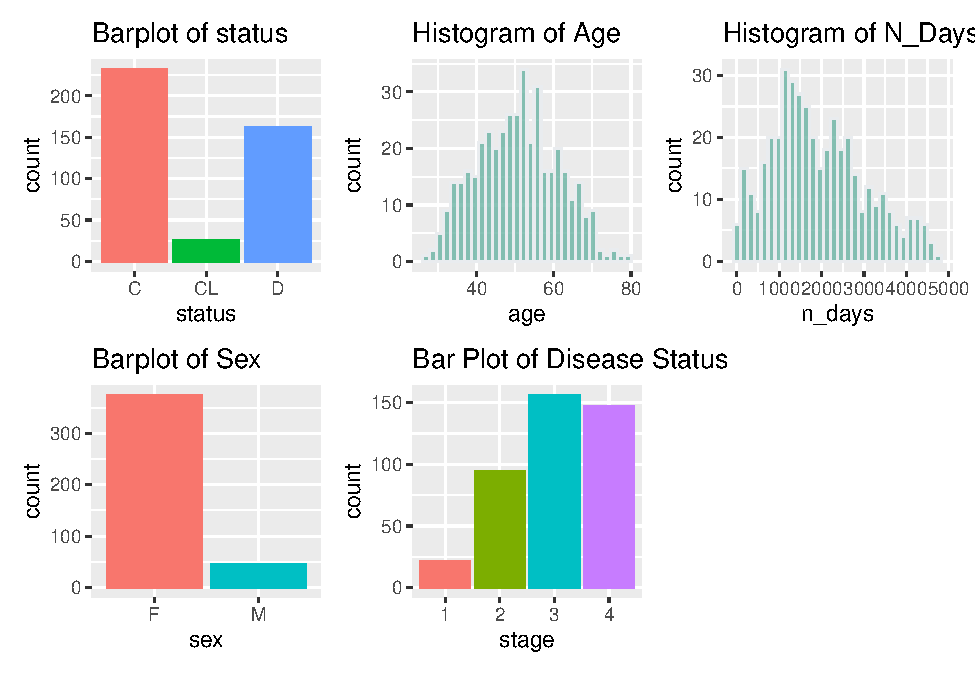
\includegraphics{final_proj_files/figure-latex/status histogram-1.pdf}

When looking at the bar plots and histogram of the status, age, and sex
respectively, we notice that a majority of the patients survived
following the treatments, however there is a significant number of
deaths as well. The patients who received transplants (denoted by CL)
are not accurate representatives of the data or the subject of this
trial and also should be dropped when analyzing the data.

Age is widely distributed but most concentrated in the 50s.

With regards to the n\_days variable, there is a larger concentration
between the 1000 and 2000 day mark which can either be attributed to
more patients dying during that time or the study ending early. This can
be explored further through a visualization relating the number of days
with the status of the patient (see below).

There are a significant number of female patients compared to male
patients which is something to note about this data--any results or
predictions are likely to be more accurate for women than men.

It looks like this drug trial happened with patients mostly in stage 3
or stage 4. This is likely because patients did not catch the diagnoses
earlier in the stage of the disease.

\begin{Shaded}
\begin{Highlighting}[]
\FunctionTok{ggplot}\NormalTok{(cholangitis, }\FunctionTok{aes}\NormalTok{(}\AttributeTok{x=}\NormalTok{status, }\AttributeTok{y=}\NormalTok{n\_days)) }\SpecialCharTok{+} 
    \FunctionTok{geom\_boxplot}\NormalTok{(}\AttributeTok{fill=}\StringTok{"slateblue"}\NormalTok{, }\AttributeTok{alpha=}\FloatTok{0.2}\NormalTok{)}
\end{Highlighting}
\end{Shaded}

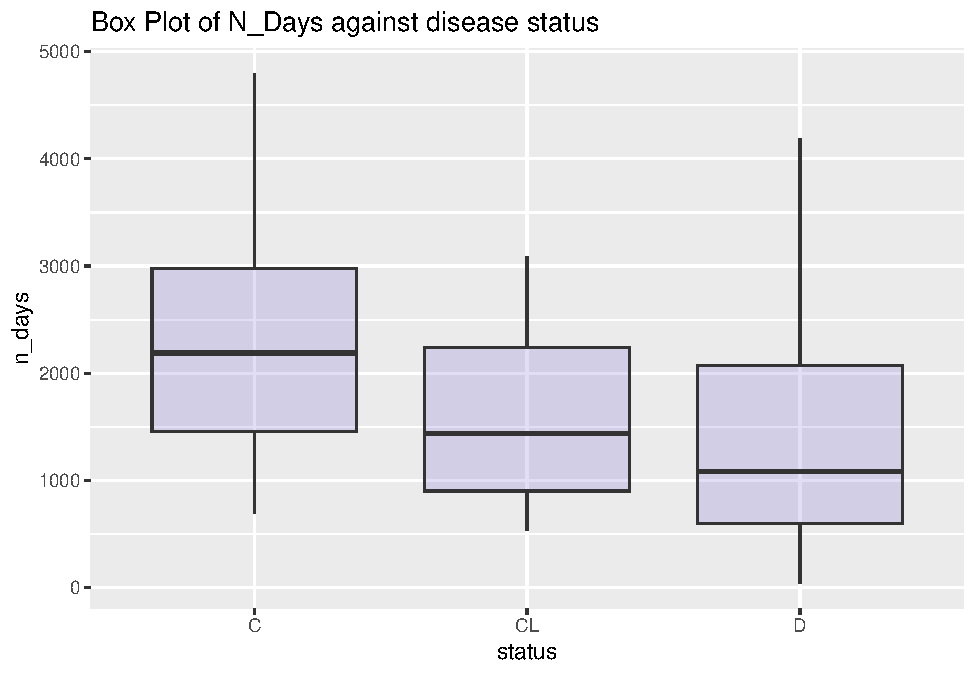
\includegraphics{final_proj_files/figure-latex/n_days and status-1.pdf}
From this boxplot, the median date for patients who died is around 1000,
while the median release time for patients who survived was close to
2000 days. This coincides with the histogram previously seen and
suggests that a large number of patients will survive at least 1000
days.

\begin{Shaded}
\begin{Highlighting}[]
\FunctionTok{mosaicplot}\NormalTok{(drug}\SpecialCharTok{\textasciitilde{}}\NormalTok{status, cholangitis)}
\end{Highlighting}
\end{Shaded}

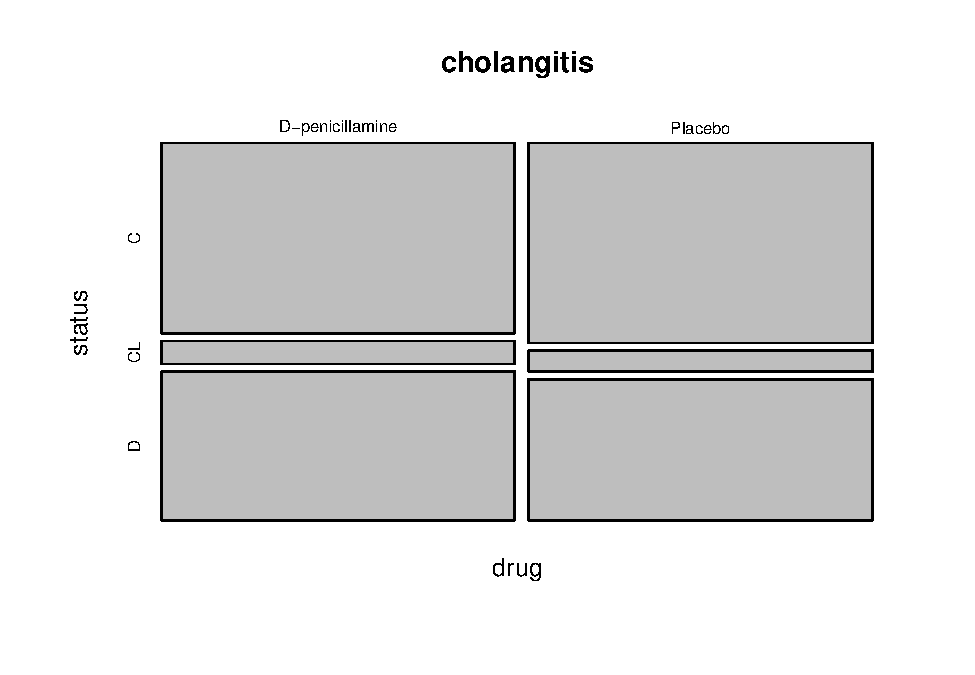
\includegraphics{final_proj_files/figure-latex/unnamed-chunk-2-1.pdf}
Based on this mosaic plot, the ratio of people who received the placebo
that survived is higher than those who received the trial drug.

\begin{Shaded}
\begin{Highlighting}[]
\NormalTok{ascites\_bar }\OtherTok{\textless{}{-}} \FunctionTok{ggplot}\NormalTok{(cholangitis, }\FunctionTok{aes}\NormalTok{(}\AttributeTok{x=}\NormalTok{ascites, }\AttributeTok{color=}\FunctionTok{factor}\NormalTok{(ascites), }\AttributeTok{fill=}\FunctionTok{factor}\NormalTok{(ascites))) }\SpecialCharTok{+}
  \FunctionTok{geom\_bar}\NormalTok{() }\SpecialCharTok{+} 
  \FunctionTok{theme}\NormalTok{(}\AttributeTok{legend.position=}\StringTok{"none"}\NormalTok{)}

\NormalTok{hepatomegaly\_bar }\OtherTok{\textless{}{-}} \FunctionTok{ggplot}\NormalTok{(cholangitis, }\FunctionTok{aes}\NormalTok{(}\AttributeTok{x=}\NormalTok{hepatomegaly, }\AttributeTok{color=}\FunctionTok{factor}\NormalTok{(hepatomegaly), }\AttributeTok{fill=}\FunctionTok{factor}\NormalTok{(hepatomegaly))) }\SpecialCharTok{+}
  \FunctionTok{geom\_bar}\NormalTok{() }\SpecialCharTok{+} 
  \FunctionTok{theme}\NormalTok{(}\AttributeTok{legend.position=}\StringTok{"none"}\NormalTok{)}

\NormalTok{spiders\_bar }\OtherTok{\textless{}{-}} \FunctionTok{ggplot}\NormalTok{(cholangitis, }\FunctionTok{aes}\NormalTok{(}\AttributeTok{x=}\NormalTok{spiders, }\AttributeTok{color=}\FunctionTok{factor}\NormalTok{(spiders), }\AttributeTok{fill=}\FunctionTok{factor}\NormalTok{(spiders))) }\SpecialCharTok{+}
  \FunctionTok{geom\_bar}\NormalTok{() }\SpecialCharTok{+} 
  \FunctionTok{theme}\NormalTok{(}\AttributeTok{legend.position=}\StringTok{"none"}\NormalTok{)}

\NormalTok{edema\_bar }\OtherTok{\textless{}{-}} \FunctionTok{ggplot}\NormalTok{(cholangitis, }\FunctionTok{aes}\NormalTok{(}\AttributeTok{x=}\NormalTok{edema, }\AttributeTok{color=}\FunctionTok{factor}\NormalTok{(edema), }\AttributeTok{fill=}\FunctionTok{factor}\NormalTok{(edema))) }\SpecialCharTok{+}
  \FunctionTok{geom\_bar}\NormalTok{() }\SpecialCharTok{+} 
  \FunctionTok{theme}\NormalTok{(}\AttributeTok{legend.position=}\StringTok{"none"}\NormalTok{)}

\NormalTok{ascites\_bar }\SpecialCharTok{+}\NormalTok{ hepatomegaly\_bar }\SpecialCharTok{+}\NormalTok{ spiders\_bar }\SpecialCharTok{+}\NormalTok{ edema\_bar}
\end{Highlighting}
\end{Shaded}

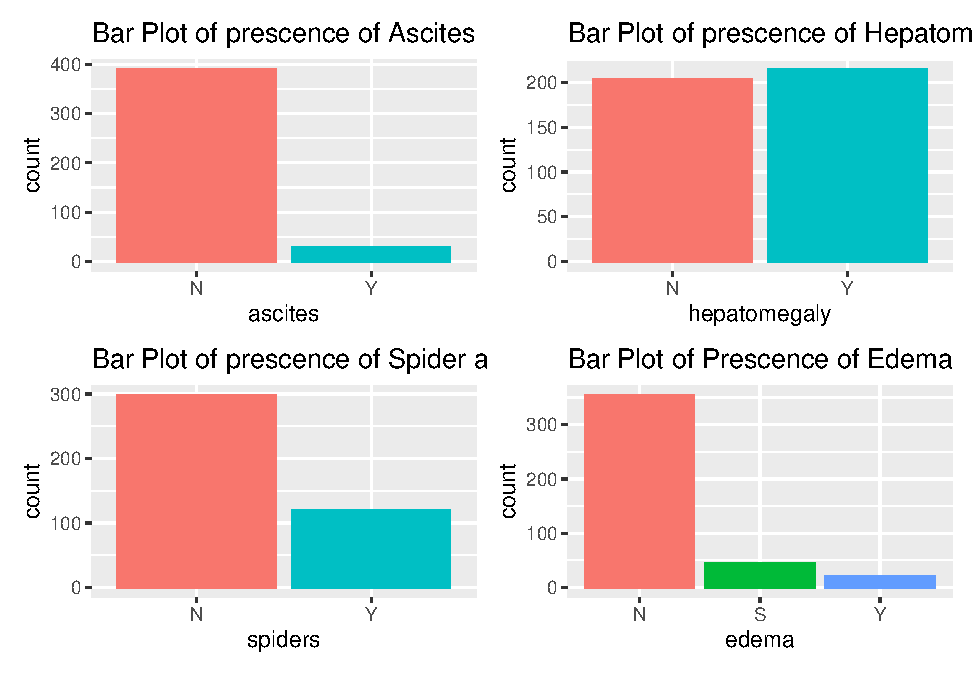
\includegraphics{final_proj_files/figure-latex/medical indicators bar plot-1.pdf}
Based on these plots, a majority of the patients did not have a presence
of spider angiomas or ascites. There was essentially an even balance of
patients who had and did not have hepatomegaly. A majority of patients
did not have edema nor have diuretic therapy.

\begin{Shaded}
\begin{Highlighting}[]
\NormalTok{chol\_continuous }\OtherTok{\textless{}{-}} \FunctionTok{select}\NormalTok{(cholangitis, }\SpecialCharTok{{-}}\FunctionTok{all\_of}\NormalTok{(cat\_vars))}

\FunctionTok{pairs}\NormalTok{(chol\_continuous)}
\end{Highlighting}
\end{Shaded}

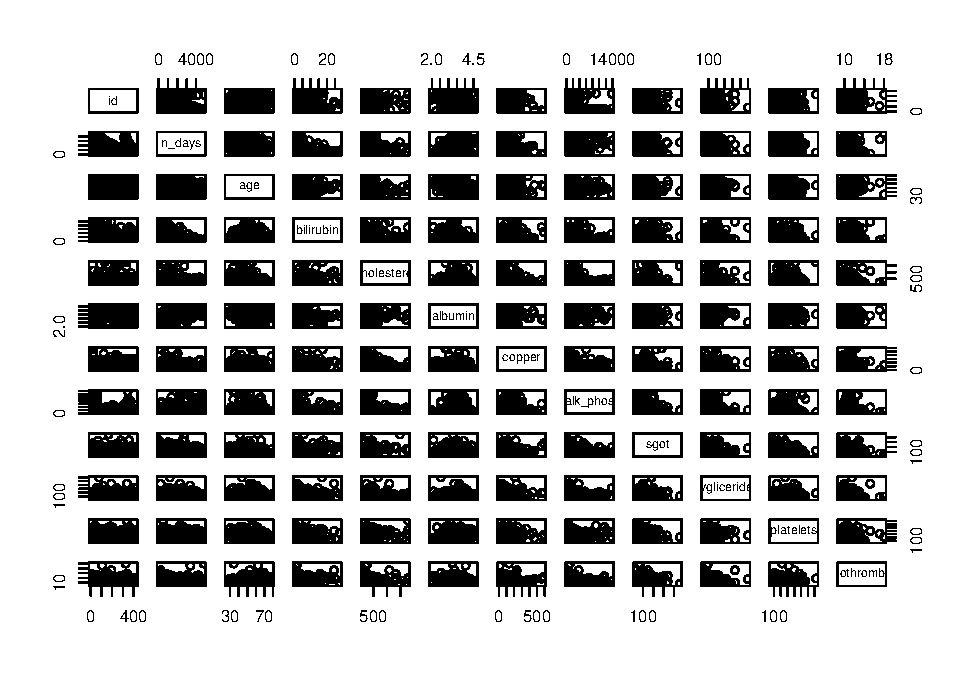
\includegraphics{final_proj_files/figure-latex/continuous-1.pdf}

\hypertarget{question-3-multivariate-regression}{%
\subsubsection{Question 3: Multivariate
Regression}\label{question-3-multivariate-regression}}

\begin{Shaded}
\begin{Highlighting}[]
\NormalTok{cholangitis\_clean }\OtherTok{\textless{}{-}}\NormalTok{ cholangitis }\SpecialCharTok{\%\textgreater{}\%} 
  \FunctionTok{subset}\NormalTok{(status }\SpecialCharTok{!=} \StringTok{"CL"}\NormalTok{)}
\end{Highlighting}
\end{Shaded}

\begin{Shaded}
\begin{Highlighting}[]
\NormalTok{continuous\_fit }\OtherTok{\textless{}{-}} \FunctionTok{lm}\NormalTok{(n\_days }\SpecialCharTok{\textasciitilde{}}\NormalTok{ ., chol\_continuous)}
\end{Highlighting}
\end{Shaded}


\end{document}
